\scanpage{10}
\[
\underline K(X\times P^r)=\underline K(X)\otimes\underline K(P^r)\quad/\quad \xi=1-L^{-1}.
\]
\diagram{\begin{tikzcd}
X \arrow[r,dash,"i"] & X\times P^r
\end{tikzcd}}
\[
F\otimes L
\]
\[
i_!(x)=p^!(x)\otimes q^!(\xi^r)=x\otimes\xi^r
\]
\[
\widetilde C(i_!(x))=\widetilde C(x\otimes\xi^r)=\widetilde C(x)*\widetilde C(\xi^r)
\]
\figure{\begin{tikzpicture}[x=1cm,y=1cm]
\node[anchor=west] at (0,0) {$\displaystyle\xi^r=\sum_{i=0}^r\binom ri(-1)^iL^{-i}$};
\node at (3.2,.75) {$\deleted{\widetilde C}$};
\draw (-.2,.62) .. controls (1.4,.54) and (3.7,.93) .. (5.5,.82);
\draw (-.15,.15) -- (.38,-1.05);
\end{tikzpicture}}

\diagram{\begin{tikzcd}
\underline K(X) \arrow[r,"\text{\uuline{injectif}}"] \arrow[d,"\widetilde C_X"'] & \underline K(X\times P^r) \arrow[d,"\widetilde C_{X\times P^r}"]\\
\widetilde A(X) \arrow[r] & \widetilde A(X\times P^r)
\end{tikzcd}}
\[
p^{\deleted{\unsure{!}}}_*i_*(x)=(pi)_*x=x
\]
\figure{\begin{tikzpicture}[x=1cm,y=1cm]
\node[anchor=west] at (5.3,0) {$\displaystyle\widetilde C(\xi^r)=\prod_{i=0}^r(1-i\eta)^{(-1)^i\binom ri}$};
\node[anchor=west] at (5.0,-1.5) {$\displaystyle\widetilde C(i_!(x))=\prod_{i=0}^r[\widetilde C(x)*(1-i\eta)]^{(-1)^i\binom ri}$};
\node[anchor=west] at (6.9,-2.8) {$\deleted{=\displaystyle\prod_{i=0}^r\bigl[(1-i\unsure{\xi|\eta})^{\varepsilon(x)}\sum_{i=0}^\infty C^i(x)}$};
\draw (5.35,.65) -- (12.9,1.0);
\draw (5.15,.48) .. controls (5.1,-1.4) and (5.23,-2.9) .. (5.45,-3.55);
\draw (12.88,.64) .. controls (13.05,-.2) and (12.8,-2.2) .. (12.6,-2.9);
\draw (7.3,-3.28) .. controls (8.9,-3.25) and (11.7,-3.2) .. (13.3,-3.0)
 .. controls (13.8,-2.9) and (13.7,-3.2) .. (13.3,-3.3)
 -- (9.65,-4.0) .. controls (9.1,-4.1) and (11.2,-6.7) .. (11.55,-7.25)
 .. controls (11.75,-7.65) and (11.8,-8.1) .. (11.45,-8.2)
 -- (7.6,-8.25) .. controls (7.0,-8.2) and (7.25,-7.7) .. (7.35,-7.35);
\draw (0,-3.85) .. controls (2.8,-4.0) and (6.8,-3.45) .. (8.95,-3.55);
\node[anchor=west] at (.55,-4.25) {$\displaystyle\widetilde C(x)*(1-i\eta)=\widetilde C(x)*[1,1-i\eta]-\widetilde C(x)$};
\node[anchor=north west] at (2.7,-4.7) {$\displaystyle=\biggl[\varepsilon(x),1+\cdots+
\underbrace{\sum_{j=0}^h C^{\unsure{j}}\deleted{\unsure{\xi}}(x)(-i\eta)^{h-j}}_{
\substack{\text{\unsure{h.ième} terme }C^h\\\text{de la série}\\\widetilde C(x)*[1,1-i\eta]}}$};
\draw (.6,-4.12) -- (.6,-5.75) .. controls (2,-5.6) and (3.4,-5.55) .. (3.95,-5.9)
 .. controls (4.25,-6.1) and (3.95,-6.7) .. (4.45,-6.85)
 .. controls (5.3,-7.0) and (8.1,-7.05) .. (9.7,-7.25);
\end{tikzpicture}}

\[
\widetilde C(\xi^r)=1+(-1)^{r-1}(r-1)!\eta^r
\]
d'où
\[
\widetilde C(i_!(x))=\widetilde C(x)*(1+(-1)^{r-1}(r-1)!\eta^r)
\]
\deleted{\unsure{D'où}}
\[
=\bigl(1+(-1)^{r-1}(r-1)!\eta^r\bigr)^{\varepsilon(x)}
\underbrace{\left(C(x)*\left(1+\overbrace{(-1)^{r-1}(r-1)!\eta^r}^{\alpha^r}\right)\right)}_{
1+\sum_{i=\unsure{1}}^\infty Q_i(C^1(x),\mathrel{\text{---}}C^i(x);0\mathrel{\text{---}}0\,\underset{\substack{\text{\unsure{r.ième} argument}\\\text{après le ;}}}{\uuline{\alpha^{(r)}}},0\mathrel{\text{---}}0)}
\]
\margin{$\underline O_{\unsure{Y|y}}=1-L(-\unsure{Y|y})$\\
$1-\underline O_{\unsure{Y|y}}=L(-\unsure{Y|y})$}

Or $Q_i$ n'a pas de terme ne contenant pas un des \unsure{$c^j$}.

\margin{9}
